\chapter{Probability}

\begin{problem}
	Given $N$ people in a room, what is the probability that $2$ or more people share a birthday?
\end{problem}

\begin{solution}
	This problem is an exercise in counting. First, lets go case-by-case and write out the general solution. There are 365 days in total. If there is only 1 person in the room, only 1 day is taken. Once we place the second person in the room, we can calculate the probability of the two individuals not-sharing the same birthday;
	\begin{equation}
		\mathbb{P}[\textbf{share birthday}] = 1 - \mathbb{P}[\textbf{ not share birthday}]
	\end{equation}
	Ie, the second person has only $364$ days to choose from to not share. Thus, their probability of not sharing a birthday are $364/365$, ie the event space over the sample space. Likewise, the following person has now only $363$ days to choose from and so on. This relation can be multiplied together such that the overall probability of not sharing is that nobody in the room is sharing. This can be built using a product;
	\begin{equation}
		\mathbb{P}[\textbf{not share birthday}] = \prod_{x=1}^N \frac{365 - x}{365}
	\end{equation}
	This gives us the probability that at least 2 people are sharing;
	\begin{equation}
		\mathbb{P}[\textbf{at least 2 share birthday}] = 1 - \prod_{x=1}^N \frac{365 - x}{365}
	\end{equation}
	Plotting this relation as a function of $N$, we can see the shape of this relation in Fig. \ref{prob_birthday}.
	\begin{figure}[h!]
		\centering
		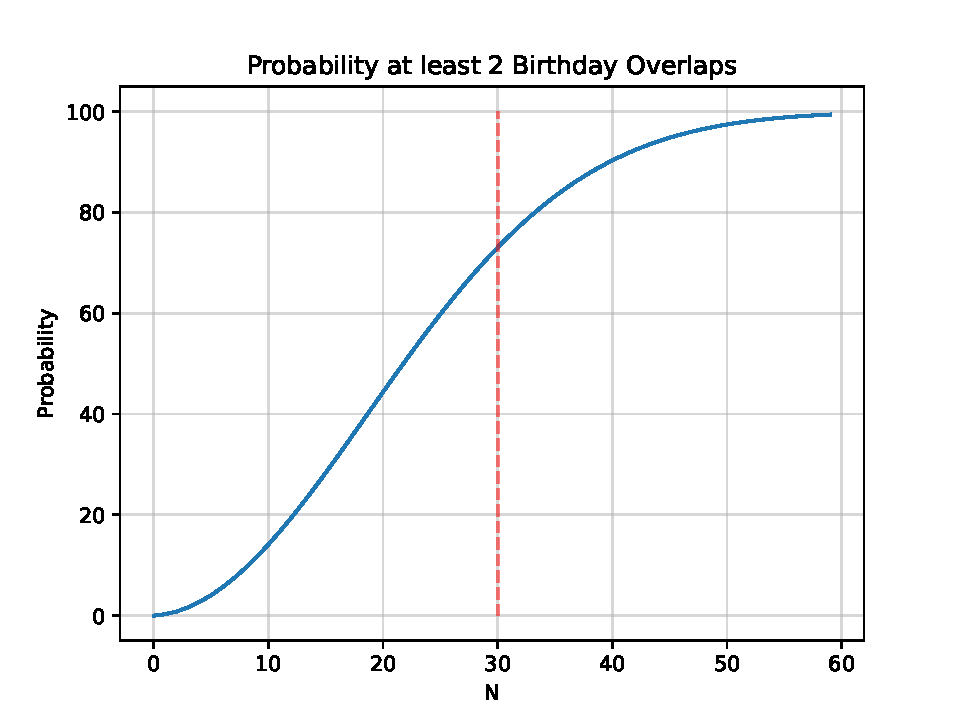
\includegraphics[width=0.75\textwidth]{figures/probability/prob_birthday.pdf}
		\caption{Probability of at least 2 people in a room sharing a birthday as a function of $N$ people in the room. at $N=30, \mathbb{P} \approx 73\%$}
		\label{prob_birthday}
	\end{figure}
\end{solution}